\chapter{Material and Methods}

\textbf{SARS-CoV 2 genome data set.} 
We create a dataset of 360 genetic sequences from December 2019 to March 8 2020, obtained from publicly available data on GISAID \cite{Shu2017} (accessed on November 2020). We follow the Nextstrain workflow for the curation of the dataset \cite{nextstrain}. Sequences with incomplete collection date, less than 27.000 bases in length or with more than 3.000 unknown bases are omitted. Also, sequences from known clusters of transmission or from the same patient are excluded. The resulting worldwide sequence dataset is aligned with MAFFT. The begining and the end of the alignment are masked respectively by 100 and 50 sequences as well as sites  13402, 24389 and 24390, identified by Nextstrain as prone to sequencing errors.

To focus on the early dynamics in Europe we select sequences from China, origin of the epidemic; France and Germany, the European countries with the earliest cases; and Italy and Spain, the European countries with the biggest outbreaks in March. To take into account the dynamics in other regions of Europe we include a group of 50 sequences from other European countries. We limit our sample of Chinese genomes to sequences until January 23, the starting date of the lockdown in Hubei. 

Due to the large (and unprecendented) number of available genetic sequences for SARS-CoV-2, we need to subsample the alignment. Each sequence is subsampled with a probability equal to the probability of having a reported case in that country the day of sample collection, inversely weighted by the probability of having a sequence in GISAID that day in the country. With this subsampling protocol, we aim to get a constant sampling proportion across the full period for each country. 

This dataset of genetic sequences is the main source of information in our phylodynamic analysis. The goal is to infer the phylogenetic tree, i.e. the evolutionary tree-shaped relationship among the sequences, together with the epidemiological transmission parameters that gave rise to it. These parameters are defined within a population dynamic model and will inform us about the epidemic that the viral genetic sequences come from.

\textbf{The multitype birth death model.} 
To study the early dynamics of SARS-CoV-2 in the European countries, we use a simplified version of the multitype birth-death model described in \cite{Kuhnert2016}, following the analysis in \cite{Nadeau2020}. Birth death models are compartmental population models with high flexibility that describe the process of epidemiological transmission. The stochastic formulation of these models are used in phylodynamic analyses \cite{Stadler2012}. In the multitype version, we consider a structured population in types or subpopulations with characteristic within-subpopulation dynamics and migrations between them. In our case, the subpopulations are the different locations of the samples.

The process starts with one infected host in one of the subpopulations, e.g in subpopulation $i$, who can infect another individual at rate $\lambda_i$, become uninfectious at rate $\mu_i$ by death or recovery, migrate to another deme $j$ at rate $m_{ij}$ or be sequenced at rate $\psi_i$ to become part of the phylogenectic tree. This process depicts the full transmission dynamics and specifically, the generation of the phylogenetic tree that we observed from our sequence data. 

Under this model, we are able to compute the likelihood of the multitype birth-death parameters for a given tree. This likelihood is derived in \cite{Kuhnert2016} by considering the probability of an individual evolved as observed in the tree. This derivation is analogous to the work in \cite{Stadler2013}, which is based on ideas from \cite{Maddison2007}.

We parameterize our model in terms of the effective reproductive number $R_i = \frac{\lambda_i}{\mu_i + \psi_i}$, a key value in epidemic control and understanding, the rate of becoming uninfectious $\delta_i = \mu_i + \psi_i$, the probability of and individual to be sequenced $s_i = \frac{\psi_i}{\mu_i + \psi_i}$ and the migration rates between locations $m_ij$.\\

\textbf{Epidemic trajectories and structured trees.} 
We will refer to the full sequence of transmissions, recoveries/deaths, migrations and sampling events as an epidemic trajectory. One set of sequences, and therefore one phylogenetic tree, is the product of one epidemic trajectory. Moreover, the tree represents a fraction of the events in the epidemic trajectory, those that involve the sampled individuals. In epidemiology, we aim to learn about the true epidemic trajectory since we usually have incomplete information caused by unreported cases or unknown transmission chains.

From the sequences metadata, we know the location of the tree tips. However, if we know the epidemic trajectory we also know the location of the lineage at any point in time in the tree. We will refer to the phylogenies with ancentral locations mapped onto the tree as structured trees \cite{Vaughan2014}. In Fig \ref{fig:epitrajs} we show the epidemic trajectories corresponding to two different subpopulations and the structured tree of a set of samples. The change of ancestral location, represented by a change in color from blue to red in the tree, is caused by a migration event from one subpopulation to the other, depicted in the epidemic trajectories.

\begin{figure}[h]
    \centering
    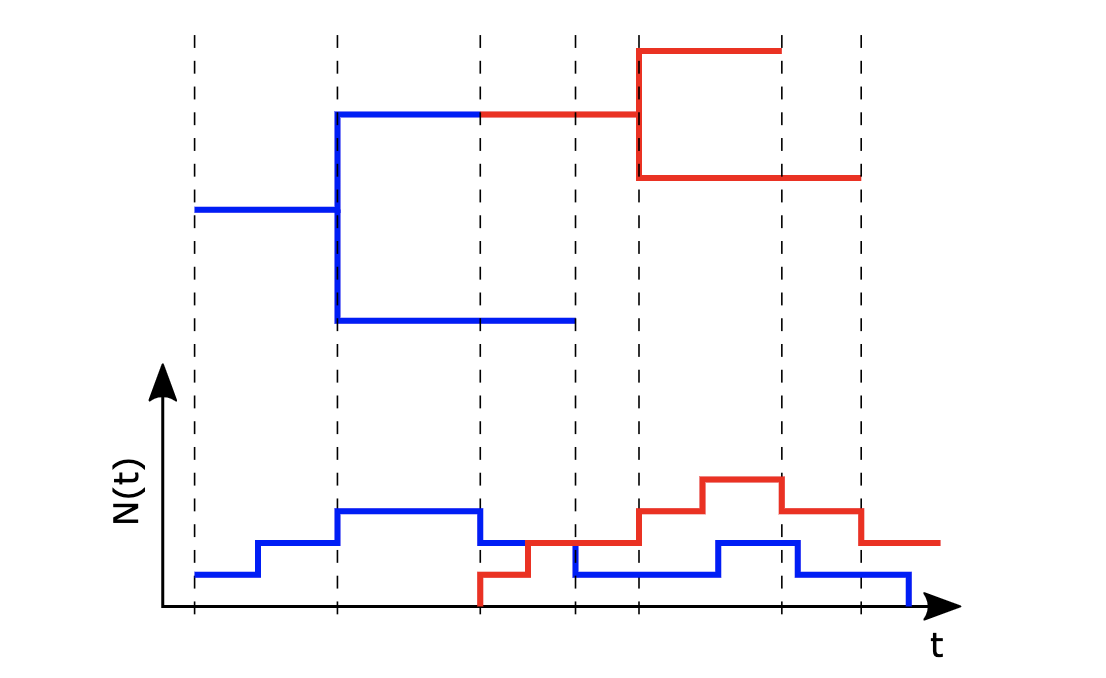
\includegraphics[width=\textwidth]{figures/epitrajs.png}
    \caption{Example of structured tree (up) and epidemic trajectories (bottom) for two types. The horizontal axis represents time, and for the epidemic trajectories the vertical axis is the population size N(t). Figure from Tim Vaughan. \todo[inline]{Use figure from EpinInf paper?}}
    \label{fig:epitrajs}
\end{figure}

\textbf{Bayesian Inference with BDMM-Prime.} 
We want to infer the epidemic trajectories under the multitype birth-death model fit to a set of samples collected throughout SARS-CoV-2 early epidemics in Europe. In order to do this, we have to estimate the joint posterior distribution of the structured tree $\mathcal{T}_c$, the epidemic trajectory $\mathcal{E}$, the substitution model parameters $\theta$ and the multi-type birth death parameters $\eta$. This posterior probability can be expressed with Bayes' formula as:

\begin{equation}
P(\mathcal{T}_c, \mathcal{E}, \theta, \eta | A ) = \frac{P(A | \mathcal{T}_c, \mathcal{E}, \theta, \eta ) P(\mathcal{T}_c, \mathcal{E}, \theta, \eta)}{P(A)}
\label{eq:posterior1}
\end{equation}

where A is the sequence alignment.

We make the following independence assumptions:

\begin{align}
P(A | \mathcal{T}_c, \mathcal{E}, \theta, \eta ) &= P(A | \mathcal{T},\theta )\\
P(\mathcal{T}_c, \mathcal{E}, \theta, \eta) &= P(\mathcal{T}_c|\mathcal{T}, \eta) P(\mathcal{E}|\mathcal{T}_c, \eta) P(\mathcal{T} | \eta ) P(\theta) P(\eta)
\label{eq:assumptions}
\end{align}


Where $\mathcal{T}$ is the rooted time tree without ancestral locations. Thus, we can express Equation \ref{eq:posterior1} in terms of the conditional distributions:

\begin{align}
P(\mathcal{T}_c, \mathcal{E}, \theta, \eta | A) &= P(\mathcal{T}_c|\mathcal{T}, \eta) P(\mathcal{E}|\mathcal{T}_c, \eta) \frac{P(A | \mathcal{T}, \theta) P(\mathcal{T} | \eta) P(\theta) P(\eta)}{P(A)}\\
&= P(\mathcal{T}_c|\mathcal{T}, \eta) P(\mathcal{E}|\mathcal{T}_c, \eta) P(\mathcal{T}, \theta, \eta | A)
\label{eq:posterior2}
\end{align}

$P(\mathcal{T}_c|\mathcal{T}, \eta)$, $P(\mathcal{E}|\mathcal{T}_c, \eta)$ and $P(\mathcal{T}, \theta, \eta | A)$ are the posterior probabilities of the structured tree, the epidemic trajectory and the joint posterior of the phylogenetic tree (without ancestral locations) and the model parameters. The tree likelihood $P(A | \mathcal{T},\theta )$ is the probability of the sequence alignment and can be efficiently evaluated using Felsenstein’s pruning algorithm \cite{Felsenstein1981}. The tree prior, $P(\mathcal{T} | \eta)$ also called phylodynamic likelihood is derived from the multitype birth-death model. $P(\theta)$ and $P(\eta)$ represent our prior belief in the distribution of the population and substitution model parameters. 

We use a Markov chain Monte Carlo (MCMC) Metropolis-Hastings algorihtm to approximate this posterior. Since the MCMC only uses ratios of posterior probabilities, we avoid calculating the marginal likelihood $P(A)$. This algorithm is implemented in BDMM-Prime package \cite{bdmmp} for BEAST 2.6.3 \cite{Bouckaert2019}. BDMM-Prime first samples from $P(\mathcal{T}, \theta, \eta | A)$, then in a second step these samples are augmented by sampling from $P(\mathcal{T}_c|\mathcal{T}, \eta)$ and $P(\mathcal{E}|\mathcal{T}_c, \eta) $ and adding these variables to obtain the overall posterior $P(\mathcal{T}_c, \mathcal{E}, \theta, \eta | A)$. In this way, $P(\mathcal{T}_c|\mathcal{T}, \eta)$ and $P(\mathcal{E}|\mathcal{T}_c, \eta) $  are only calculated for a subset of samples instead of every MCMC step.


While it is also possible to include $\mathcal{T}_c$ and $\mathcal{E}$ directly into the Bayes' rule as implemented in EpiInf package \cite{Vaughan2019}, the factorization of the posterior in these three terms allow us to use the standard birth-death-sampling tree prior implementations in BDMM to compute $P(\mathcal{T}, \theta, \eta | A)$ \cite{Kuhnert2016} \cite{Scire2020}. This will speedup the analysis with almost no overhead compared to the standard BDMM inference and can be used in pre-existing multitype analyses withoud additional MCMC.\\

\textbf{Stochastic mapping of ancestral locations and epidemic trajectories}
To sample from $P(\mathcal{T}_c|\mathcal{T}, \eta)$, BDMM-Prime implements a stochastic mapping algorithm based on the work by \cite{Hohna2019}. A set of differential equations is numerically integrated over $\mathcal{T}$ to obtain the marginal probability of a location value at any point along each branch. From this probabilities, we can derive time-dependent rates that define the changes of the location along the tree according to a continuous-time Markov process. Then, we can simulate forward in time from the root of the tree the location trajectories down the tree edges. For a detailed derivation of the stochastic mapping of the algorithm refer to \cite{VaughanWIP}.\\

In the case of $P(\mathcal{E}|\mathcal{T}_c, \eta)$, following Bayes'rule:

\begin{equation}
P(\mathcal{E}|\mathcal{T}_c, \eta) = \frac{P(\mathcal{T}_c, \eta|\mathcal{E}) P(\mathcal{E})}{P(\mathcal{T}_c, \eta)} = \frac{P(\mathcal{T}_c|\mathcal{E}) P(\mathcal{E}| \eta)}{P(\mathcal{T}_c | \eta)}
\label{trajectories}
\end{equation}

We can easily compute the probability of a structured tree for a given epidemic trajectory $P(\mathcal{T}_c|\mathcal{E})$ as described in \cite{Vaughan2019}. Each node in the structured tree must correspond to a compatible event in the epidemic trajectory for this probability to be nonzero. If we simulate an epidemic trajectory directly from $P(\mathcal{E}| \eta)$, it is very likely that the simulated events will not match with the events in the tree and $P(\mathcal{T}_c|\mathcal{E})$ will be 0. To avoid this problem, we simulate from $P^*(\mathcal{E}| \eta)$, which guarantees trajectories with non-zero probabilities by enforcing the tree events. Provided we weight these trajectories accordingly we can efficiently sample from $P(\mathcal{E}|\mathcal{T}_c, \eta)$:

\begin{equation}
P(\mathcal{E}^{(a)}|\mathcal{T}_c, \eta) = w_a^* P^*(\mathcal{E}^{(a)}| \eta) \propto P(\mathcal{T}_c | \mathcal{E}^{(a)}) \frac{P(\mathcal{E}^{(a)} | \eta)}{P^*(\mathcal{E}^{(a)} | \eta)} P^*(\mathcal{E}^{(a)}| \eta)
\label{eq:traj}
\end{equation}

The epidemic trajectories are simulated with an adaptive tau-leaping algorithm \cite{Gillespie2000} in BDMM-Prime. This method is based on the Gillespie algorithm \cite{Gillespie1977} but the simulation time is divided in small intervals and the number of events is drawn from a poisson distribution for each interval. This algorithm is more efficient that Gillespie when we have a high number of individuals since we have to update the rates less often. 

We simulate a fixed number of trajectories, called particles, for each set of population parameters $\eta$ and structured tree $\mathcal{T}_c$. The trajectories are simulated until some point and are weigthed as described in Equation \ref{eq:traj}. We resample using importance sampling to get rid of low-weighted trajectories and then resume the simulation of all the particles from the sampled trajectory ending point. This process is repeated until the end of the simulation. Then, we sample one single trajectory from the set of final trajectories with important sampling and record each event and its timing to future analysis \cite{VaughanWIP}. All these steps are implemented by BDMM-Prime trajectory logger and we use it in our analysis.\\

We conducted two different analyses. One with constant migration rates as in the standard multi-type birth death model and the other one with time-changing migration rates informed by travel data. We use the BDMM-Prime package \cite{bdmmp} implemented in BEAST 2.6.3 \cite{beast}. We run 10 parallel chains for analysis, of $10^7$ iterations each with different initial values. These chains are assesed for convergence using Tracer v.1.7.1 and then combined after removing a 10\% burnin. We check that the effective sample size (ESS) is greater than 200 for all parameters. The stochastic mapping of structured trees and epidemic trajectories is performed in a second step using the trace and tree logs from the MCMC. We use 300, 1000, 3000 and 10000 particles in the tau-leaping simulation of epidemic trajectories, and a tolerance of 0.03 for selecting tau leap length.\\


\textbf{Incorporating air travel data and geographic distances.}
 In order to inform our migration rates with external information, and to avoid having to estimate a large number of migration rates we implement a generalized linear model (GLM) for the migration matrix based on \cite{Lemey2014} and \cite{Nicola2019}. This GLM model parametrizes the migration rates as a log linear function of a number of potential predictors, Equation \ref{eq:glm}. For each predictor $x_i$, the GLM parameterization includes a coefficient $\beta_i$, which quantifies the effect size of the predictor, and a binary indicator variable $\delta_i$, that allows the predictor to be included or excluded from the model. The parameter $c$ represents the overal magnitude of migration. This means that if every indicator is 0, every migration rate will be equal to this parameter. In the MCMC, we estimate the effect size of each of the predictors, as well as their inclusion probability $\mathbb{E}[\delta_i]$.

\begin{equation}
m_{ij} = c \exp(\sum_{i = 1}^p \delta_i \beta_i xij)
\label{eq:glm}
\end{equation}

In a similar way to the GLM formulation in \cite{Lemey2020} we consider as predictors air travel data and geographical distance between locations. We define three time periods in our analysis: from the origin of the epidemic to January 23 (Hubei lockdown), from January 23 to end of February, from March 1 to March 8. The international travel during these months decreased drastically due to the increasing awareness about the SARS-CoV-2 pandemic as is shown in Figure \ref{fig:travel}. Thus, we would expect the migration rates to change during the time of the analysis. 

The air travel data is obtained from EUROSTATS transport datasets \textit{avia\_paexcc} and \textit{avia\_paincc}, in particular the passengers carried departures values for December 2019, January, February and March 2020. We compute the average daily flux of passengers for each of the time periods. The geographical distance is defined as the great circle pairwise distance between the centroids of the countries, computed based on the Natural Earth project (the 1:50m resolution version) world map 2013. The predictors are log transformed, a pseudocount is added to make all values positive, and then they are standardized, following the description in \cite{Lemey2014}.

\begin{figure}[h]
    \centering
    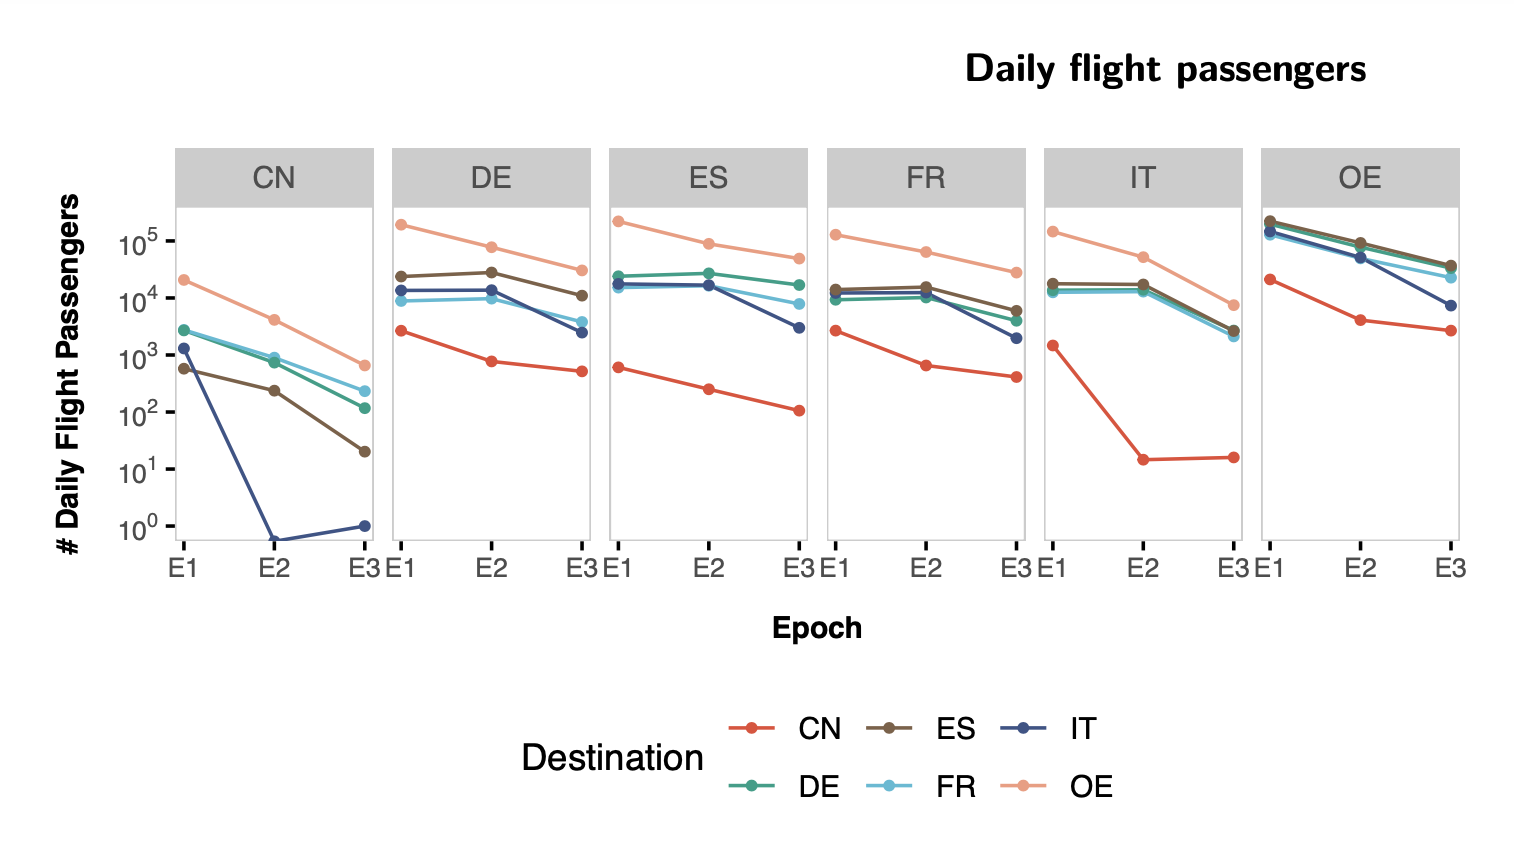
\includegraphics[width=\textwidth]{figures/flight_data.png}
    \caption{\todo[inline]{improve figure}}
    \label{fig:epitrajs}
\end{figure}

\textbf{Model specifications and priors.} 
Since we focus on the early epidemic outbreak, we expect un unimpeded spread of the virus that can be described by the exponential growth of the infected population and no significant decrease in the number of susceptibles over time \cite{Boskova2014}. Thus, we assume a constant basic reproductive number $R_0$ for each of the European countries before the lockdown in the Lombardy region in March 8. However, in China the first wave of the epidedmic had almost concluded in March so we can not make the same assumption. We fixed the reproductive number in China and include three different periods, changing on January 23 and February 10 based on \cite{Pan2020} \cite{Wu2020} \cite{Xiao2020}. Before January 23, we use the estimation in \cite{Park2020} \cite{Billah2020} to fix the basic reproductive number $R_0$ in China to $2.9$ . From January 23 to February 10 and from February 11 to March 8, we calculate the average effective reproductive number based on the estimations in \cite{covidre} \cite{Huisman2020} and obtain the $R_e$ in China to be $1.1$ and $0.43$ respectively.   

In Table \ref{table:priors} we show the values and prior distributions used in the Bayesian inference of the multitype birth death model and substitution parameters. Several of these model specifications are identical to those from \cite{Nadeau2020}.

\renewcommand{\arraystretch}{1.2}
\begin{table}[h]
\footnotesize
\begin{tabular}{@{}lll@{}}
\toprule
\textbf{Parameter}  & \textbf{Value or Prior} & \textbf{Rationale}                                              \\ \hline
\begin{tabular}[c]{@{}l@{}}Nucleotide substitution \\ model\end{tabular} &
  HKY + Gamma &
  \begin{tabular}[c]{@{}l@{}}Unequal transition/transversion rates, \\ unequal base frequencies, rate\\ heterogeneity among sites with 4 categories\end{tabular} \\
Clock rate          & 0.0008                  & Approximatelly 24 mutations per year \textbackslash{}cite\{10\} \\
Location of origin  & Hubei                   & Putative pandemic origin                                        \\
Time of origin      & Lognormal (-1, 0.2)     & \begin{tabular}[c]{@{}l@{}}Median 26 October, 95\% IQR 22 August \\ to 8 December 2019 \end{tabular}       \\
\begin{tabular}[c]{@{}l@{}}European countries \\ reproductive number\end{tabular} &
  Lognormal (0.8, 0.5) &
  Median 2.2, 95\% IQR 0.8 to 5.9 \\
\begin{tabular}[c]{@{}l@{}}China reproductive \\ number\end{tabular} &
  \begin{tabular}[c]{@{}l@{}}Origin - Jan 23: 2.9\\ Jan 23 - Feb 10: 1.1\\ Feb 11 - Mar 8:  0.43\end{tabular} &
  Fixed based on \textbackslash{}cite\{\}. \\
\begin{tabular}[c]{@{}l@{}}Becoming uninfectious \\ rate \end{tabular} &
  36.5 y-1 &
  \begin{tabular}[c]{@{}l@{}}Period between infections and becoming \\ uninfectious assumed exponentially \\ distributed with a mean of 10 days\end{tabular} \\
Sampling proportion &                         & Upper bounds based on reported cases:                           \\
China               & Uniform (0, 0.12)       &                                                                 \\
France              & Uniform (0, 0.07)       &                                                                 \\
Germany             & Uniform (0, 0.07)       &                                                                 \\
Italy               & Uniform (0, 0.01)       &                                                                 \\
Spain               & Uniform (0, 0.08)       &                                                                 \\
Other European      & Uniform (0, 0.03)       &                                                                 \\
Sampling start date & December 23, 2019       & Just before first sample from China                             \\
\begin{tabular}[c]{@{}l@{}}Sampling end date \\ (only China)\end{tabular} &
  January 23, 2020 &
  \begin{tabular}[c]{@{}l@{}} Only included Chinese sequences before \\ Lockdown in Hubei \end{tabular} 		\\ 

\begin{tabular}[c]{@{}l@{}}Migration rates \\ (no GLM analysis)\end{tabular} & Lognormal(0,1) & Median, IQR                            \\
\begin{tabular}[c]{@{}l@{}}Migration rates \\ (GLM analysis)\end{tabular} & Uniform(0,50) & \begin{tabular}[c]{@{}l@{}}7.3 days as mean of exponential time \\ to travel for every individual \end{tabular}\\
\begin{tabular}[c]{@{}l@{}}Migration rates \\ change times \\(GLM analysis)\end{tabular} & December 23, 2019 and March 1, 2020       & \\
\begin{tabular}[c]{@{}l@{}}Global scaler \\ GLM parameter\end{tabular} & December 23, 2019 & Median, IQR                              \\
\begin{tabular}[c]{@{}l@{}}Coefficients \\ GLM predictors\end{tabular} & Normal (0, 2) & Median 0, IQR                            							\\
\begin{tabular}[c]{@{}l@{}}Binary indicators \\ GLM predictors\end{tabular} & 0 - 1 equiprobable & BitFlipOperator.  			\\

\bottomrule
\end{tabular}
\caption{Caption \todo[inline]{finish table and caption}}
\label{table:priors}
\end{table}

\textbf{Data availability.}
The SARS-CoV-2 genetic data can be downloaded from www.gisaid.org \cite{Shu2017}. Supplementary Table \ref{stable:seqs} \todo{todo} lists accession numbers for the genetic sequences used in this study. Reported SARS-CoV-2 case counts are obtained from the country official agencies indicated in Table \ref{table:cases} \todo{todo}. Flight data can be obtained from EUROSTATS https://ec.europa.eu/eurostat/.

\textbf{Code availability and analyses reproducibility.}
All the code is available at ...
To ensure the reproducibility of the analysis, we have implemented the whole workflow with Snakemake \cite{snakemake}. The workflow is a modified version of Nextrain workflow \cite{nextstrain} with the additional rules for BEAST 2 analysis and results processing. 

